\documentclass[aspectratio=169,11pt]{beamer}
\usepackage[T1]{fontenc}
\usepackage{booktabs}
\usepackage{graphicx}
\graphicspath{{./}{slides/}}
\renewcommand{\familydefault}{\sfdefault}
\definecolor{accent}{HTML}{1F2A44}
\definecolor{ink}{HTML}{222222}
\setbeamercolor{normal text}{fg=ink,bg=white}
\setbeamercolor{frametitle}{fg=accent,bg=white}
\setbeamercolor{title}{fg=accent,bg=white}
\setbeamercolor{itemize item}{fg=accent}
\setbeamerfont{frametitle}{series=\bfseries,size=\Large}
\setbeamertemplate{navigation symbols}{}
\setbeamertemplate{headline}{}
\setbeamertemplate{itemize item}{--}
\setbeamertemplate{footline}{\hfill\insertframenumber\hspace{1em}\vspace{0.8em}}
\title{Can a Self-Supervised Bird Foundation Model Transfer to Soundscapes? Bird-MAE on BirdCLEF+ 2025}
\subtitle{SC4000 late submissions: a diagnostic study}
\author{Author One, Author Two, Author Three, Author Four}
\institute{Nanyang Technological University}
\date{}
\begin{document}
\begin{frame}[plain]
\titlepage
\end{frame}
\addtocounter{framenumber}{-1}

\begin{frame}{Question: do SSL foundation models transfer?}
\begin{itemize}
\item Pretrain once, freeze, train a small head
\item Bird-MAE: masked autoencoder on bird audio
\item Do frozen features transfer to field soundscapes?
\item Diagnostic study, not a bid to win
\item Limited search: no prior report found
\end{itemize}
\note{Foundation models promise a simple recipe: pretrain once on large audio collections, freeze the encoder, and train only a small head. Self-supervised learning is attractive in bioacoustics, because unlabelled recordings are plentiful, while species labels, especially for continuous soundscapes, are expensive. Bird-MAE is a masked autoencoder pretrained on bird recordings. Our question is whether its frozen features transfer to field soundscapes when the head sees only clean focal clips. We treat this as a diagnostic study, not a bid to win. We asked what the number means. In a limited search, we found no prior report of frozen Bird-MAE-Base on this competition. The practical promise is that a frozen encoder and a light head could replace expensive end-to-end training. Next, the task and its constraints.}
\end{frame}

\begin{frame}{Task and constraints}
\begin{itemize}
\item 206 classes; about 700 one-minute soundscapes
\item Predict every 5 s window; macro ROC-AUC
\item Train on focal clips, test on field audio
\item CPU only, no internet, 90 min (our budget: 75)
\item Baseline v2: public 0.763, private 0.789
\end{itemize}
\note{BirdCLEF+ 2025 asks for the species present in every five-second window of one-minute soundscapes from Colombia. There are 206 classes: 146 birds, 34 amphibians, 17 insects and nine mammals. The metric is macro ROC-AUC, skipping classes with no positives. Training data are mostly short single-species focal clips, while test data are continuous field recordings with wind, rain and overlapping calls. The submission notebook runs on CPU only, with internet off, for at most 90 minutes; our own budget is 75. We used late submissions, which are not ranked. Our baseline, v2, is an EfficientNet-B0 that scored 0.763 public and 0.789 private. A model that separates species well on clean clips may not do so under these conditions. Next, the Bird-MAE pipeline.}
\end{frame}

\begin{frame}{Method: Bird-MAE pipeline}
\begin{itemize}
\item Input: 5 s window, 32 kHz, 128-bin filterbank
\item Frozen ViT-B/16 encoder, 85.5M parameters
\item Mean of 256 patch tokens: 768-d vector, cached once
\item Heads: linear, or MLP (512 units, dropout 0.2)
\item Same split and targets as v2
\end{itemize}
\note{Audio is cut into five-second windows at 32 kilohertz. Bird-MAE's own feature extractor builds a 128-bin filterbank of 512 frames, which gives 256 patches. The encoder is a ViT-B/16 with 85.5 million parameters, and it stays frozen. We take the mean of the patch tokens, a 768-dimensional vector per window, and cache it to disk once. That took about 0.3 GPU hours on a T4. Two heads are then trained from the cache: a linear layer, and an MLP with 512 hidden units and dropout 0.2. Targets are 1.0 for primary and 0.5 for secondary labels, on v2's split. We called the extractor once per window, so each input is independent of its neighbours. Next, the first result, which looked bad.}
\end{frame}

\begin{frame}{A linear probe that looked poor}
\begin{itemize}
\item Linear probe: 0.7495 validation AUC (retry 0.7498)
\item Suggests weak pooled features
\item But loss started at 0.6929, near $\ln 2$
\item Loss plateaued at 0.277
\item Plateau points at the output offset
\end{itemize}
\note{The first linear probe reached 0.7495 validation AUC, and a retry gave 0.7498. The usual reading is that pooled features are a weak interface, which would suggest poor features. But the training loss told a different story. It started at 0.6929, close to ln 2, the loss of predicting probability one half everywhere. It then fell slowly to a plateau of 0.277. A head that had merely learned the class base rates would reach a far lower loss. So the plateau says the output offset had not been learned; it says little about the features themselves. That made us suspect the optimiser and the bias. Nothing here says the features are bad; the number simply needs explaining. Next, the sweep that pointed there.}
\end{frame}

\begin{frame}{Sweep and bias diagnosis}
\begin{minipage}[c]{0.40\textwidth}
\begin{itemize}
\item Default bias near 0; needs about $-5.3$ (uniform estimate), measured $-6.20$
\item Moves about 1.3 at LR $10^{-3}$ (analytical estimate)
\item Log-prior bias: 0.9626
\end{itemize}
\end{minipage}\hfill
\begin{minipage}[c]{0.56\textwidth}
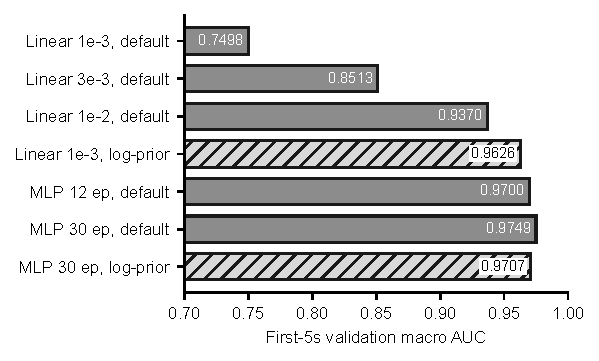
\includegraphics[width=\textwidth]{figures/diagnostic_arc.pdf}
\end{minipage}
\note{Raising the linear learning rate to 0.003 and 0.01 lifted AUC to 0.8513 and 0.9370, so step size mattered. The default bias starts near zero. A uniform-class estimate puts the right value near minus 5.3, and the measured mean log-prior is minus 6.20. A code review estimated that at learning rate 0.001 an Adam-style update moves a bias by only about 1.3 in total. That is an analytical estimate, not a measurement. Changing only the bias to the log-prior gave 0.9626, and the first-epoch loss fell from 0.6941 to 0.0285. This is one seed, so it supports the diagnosis without proving it. The same features, the same data and the same learning rate gave two very different answers. Next, the MLP heads.}
\end{frame}

\begin{frame}{MLP heads}
\small
\begin{tabular}{lc}
\toprule
MLP head & First-5s AUC \\
\midrule
12 epochs, default bias & 0.9700 \\
30 epochs, default bias & \textbf{0.9749} \\
30 epochs, log-prior bias & 0.9707 \\
\bottomrule
\end{tabular}
\begin{itemize}
\item Log-prior did not help the MLP
\item Submitted: 30-epoch default-bias head
\end{itemize}
\note{An MLP can supply its own offset. With 12 epochs it reached 0.9700, and with 30 epochs 0.9749, a gain of 0.0049. We then tried the log-prior bias on the MLP. It reached 0.9707, which is 0.0042 lower than the default. So the fix that rescued the linear probe did not help the MLP. The default-bias head won on validation, and it is the one we submitted. One possible explanation is that the hidden layer can supply a large negative offset, but we did not test it. Epoch counts differ between the sweep rows, so read that comparison with care. Retraining both heads on CPU took under two minutes each. Next, what the leaderboard said.}
\end{frame}

\begin{frame}{Leaderboard}
\begin{minipage}[c]{0.42\textwidth}
\begin{itemize}
\item A3: 0.77640 public, 0.78016 private
\item Public +0.013 vs v2: near noise (0.01)
\item Cut-off margin 0.0004: noise
\item Private $-0.009$: no improvement claimed
\end{itemize}
\end{minipage}\hfill
\begin{minipage}[c]{0.54\textwidth}
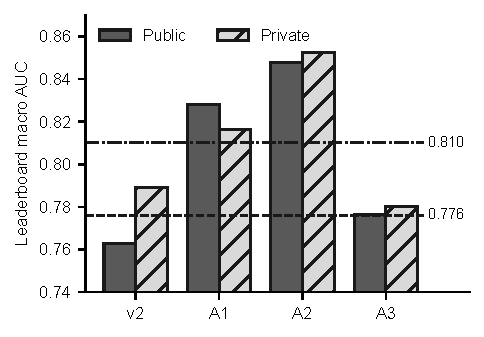
\includegraphics[width=\textwidth]{figures/leaderboard_compare.pdf}
\end{minipage}
\note{We submitted the default-bias MLP once. It scored 0.77640 public and 0.78016 private. The public gain over v2 is plus 0.013, only slightly above our 0.01 noise threshold. It clears the 0.776 cut-off by 0.0004, which is noise. The private score is 0.009 below v2, so we claim no improvement. For reference, A1, the bird-pretrained EfficientNetV2-S, scored 0.82822 and 0.81642. A2, frozen Perch 2.0 with an MLP head, scored 0.84774 and 0.85226. Perch 2.0 was released after the competition closed, so A2 is not comparable to official ranks. No ensemble was tested, and we make no ranking claim. Next, the gap between validation and leaderboard.}
\end{frame}

\begin{frame}{Transfer gap}
\begin{minipage}[c]{0.40\textwidth}
\begin{itemize}
\item Gap (public): A3 0.1985, A1 0.1550, A2 0.1439
\item Validation spread 0.017; public spread 0.071
\item Single seed, single split
\item Mixes domain shift with class coverage
\end{itemize}
\end{minipage}\hfill
\begin{minipage}[c]{0.56\textwidth}
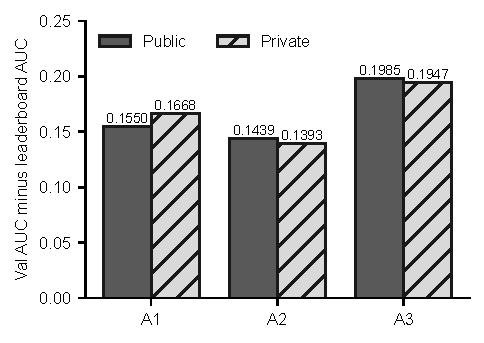
\includegraphics[width=\textwidth]{figures/transfer_gap.pdf}
\end{minipage}
\note{Subtracting leaderboard AUC from validation AUC gives the transfer gap. For Bird-MAE it is 0.1985 on the public split, against 0.1439 for Perch and 0.1550 for the CNN. Validation spans only 0.017 across the three models, while public scores span 0.071. The caveats matter. This is a single seed and a single split. Validation covers focal clips and the leaderboard covers soundscapes with a different class set, so the gap mixes domain shift with class coverage. A2's validation may also be inflated by data overlap. We read the gap as descriptive only. Bird-MAE's gap was the largest on both splits, 0.1947 on the private one. Next, three hypotheses for why Bird-MAE transferred worse.}
\end{frame}

\begin{frame}{Why? Three untested hypotheses}
\begin{itemize}
\item \textbf{H1} mean pooling dilutes short calls. Test: attention or max pooling, prototypical probe
\item \textbf{H2} head saw only clean features. Test: noise-augmented embeddings
\item \textbf{H3} pretraining objective and data. Test: labelled soundscape subset
\item A2 also used clean features: H2 alone cannot explain the gap
\end{itemize}
\note{We offer three hypotheses, and none has been tested. H1: mean pooling dilutes short calls. The test is to replace it with attention or max pooling, or a prototypical probe, over cached patch tokens. H2: the head saw only clean-clip features. The test is to embed focal clips with soundscape noise mixed in, and retrain. But A2 was also trained on clean features and transferred best, so H2 alone cannot explain the difference. H3: the pretraining objective and data differ, label-free versus supervised. The test needs a labelled soundscape subset for per-taxon AUC. The hypotheses may also interact. Each hypothesis also has a reason it might be wrong, which we give in the paper. Next, cost and practical lessons.}
\end{frame}

\begin{frame}{Cost and practical lessons}
\begin{itemize}
\item Embedding: 691 s on a T4, about 0.3 GPU h
\item CPU: 5.25 s per file; 61.6 min projected for 700 files
\item A2 25.0 min, A1 about 37 min (projected)
\item Check first-epoch loss against $\ln 2$
\item Do not rank encoders by clean validation AUC
\end{itemize}
\note{Embedding 106,157 windows took 691 seconds on a T4, about 0.3 GPU hours by our estimate. CPU inference was the slowest of our three models. A 20-file dry run took 5.25 seconds per file with four workers, which projects to 61.6 minutes for 700 files. That is a projection, not a scored-run measurement. Perch projects to 25.0 minutes and A1 to about 37, so Bird-MAE leaves the least headroom for an ensemble. Two lessons stand out. First, check the first-epoch loss against ln 2. Second, do not rank encoders by clean validation AUC, which compressed a 0.071 public spread into 0.017. Summed over workers, the encoder took 313.6 seconds against 100.9 for the mel front end. Next, limitations and conclusion.}
\end{frame}

\begin{frame}{Limitations, future work, conclusion}
\begin{itemize}
\item One seed, one split, one submission per model
\item Hypotheses untested; no prototypical probe
\item Perch logistic head plateau 0.278: presumed same defect, not re-tested
\item Next: pooling ablation, noisy embeddings, per-taxon AUC
\item Bird-MAE + MLP: no clear gain over v2
\end{itemize}
\note{The evidence rests on one seed, one split and one submission per model, so there are no error bars. The hypotheses are untested, the only causal result is the bias one, and we did not run a prototypical probe. The Perch logistic regression plateaued at 0.278, which we presume has the same defect, but we did not re-test it. Future work follows the hypotheses: a pooling ablation, noise-augmented embeddings and per-taxon evaluation. In conclusion, frozen Bird-MAE with an MLP scored 0.77640 public and 0.78016 private, no clear improvement on v2 and well below Perch. A linear probe at 0.75 reached 0.96 once its bias was corrected, so check the diagnosis before judging features. The Bird-MAE weights carry no declared licence, so we kept them private. Thank you; we welcome questions.}
\end{frame}

\end{document}
